\subsection{Implemented collection and observed access}

The new plan contains 106 inherited practitioner/lineage/partial-name candidates, 590 planned keyword queries, 157 planned account crawls and 215 proposed caption candidates, alongside 925 retained upload IDs. These are different units and are not additive. The recorded initial preflight attempted 1 ordinary watch request and observed 1 policy block; newly successful collection operations total 0. Therefore no new search results, channel histories, metadata records or captions are added by this collection phase.

The installed collector dependencies are \texttt{yt-dlp 2026.10.21} and \texttt{youtube-transcript-api 1.2.4}. The observed watch preflight used Python standard-library \texttt{urllib}; no successful tool-backed crawl or caption retrieval occurred. Package import and dependency checks establish local availability, while mocked safety tests establish selected control behavior; neither is successful platform retrieval. The documented query forms are quoted practitioner name with \emph{channeling}, \emph{questions answers}, or \emph{interview}, plus documented name/entity combinations. Other spelling variants are proposed sensitivity checks.

\subsection{Coverage and publisher concentration}

Of 925 retained uploads, 886 resolve to 180 nonempty publisher groups, while 39 remain unresolved. The largest ten groups contribute 38.04\% of attributed uploads; the largest twenty contribute 66.93\%. Thus the exploratory direction check that the largest ten exceed half is disconfirmed in this sample. These checks were recorded after inspection of the schema and prior summaries, before the new computations; they are not preregistered. The upload-count Gini is 0.671; inverse-Herfindahl effective representation is 40.30 equally sized groups. These are sample concentration measures, not audience or practitioner statistics.

\begin{figure}[p]
\centering
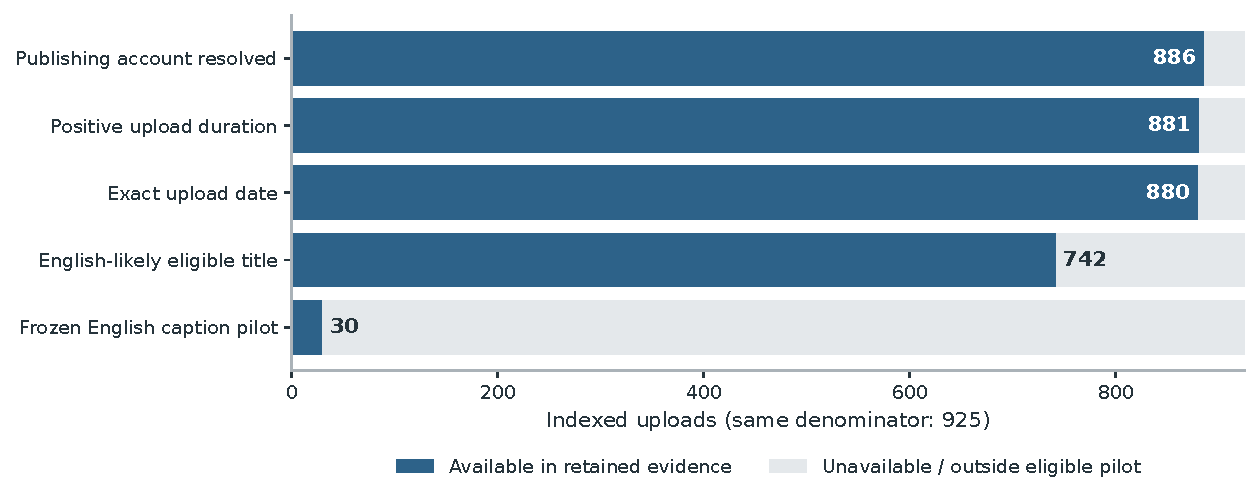
\includegraphics[width=\textwidth]{generated/figures/coverage.pdf}
\caption{Availability of retained measurement layers. The selected caption-pilot row is inclusion in this released pilot, not a census of offered-caption availability. Missing observations are not negative content findings.}
\label{fig:coverage}
\end{figure}

\begin{figure}[p]
\centering
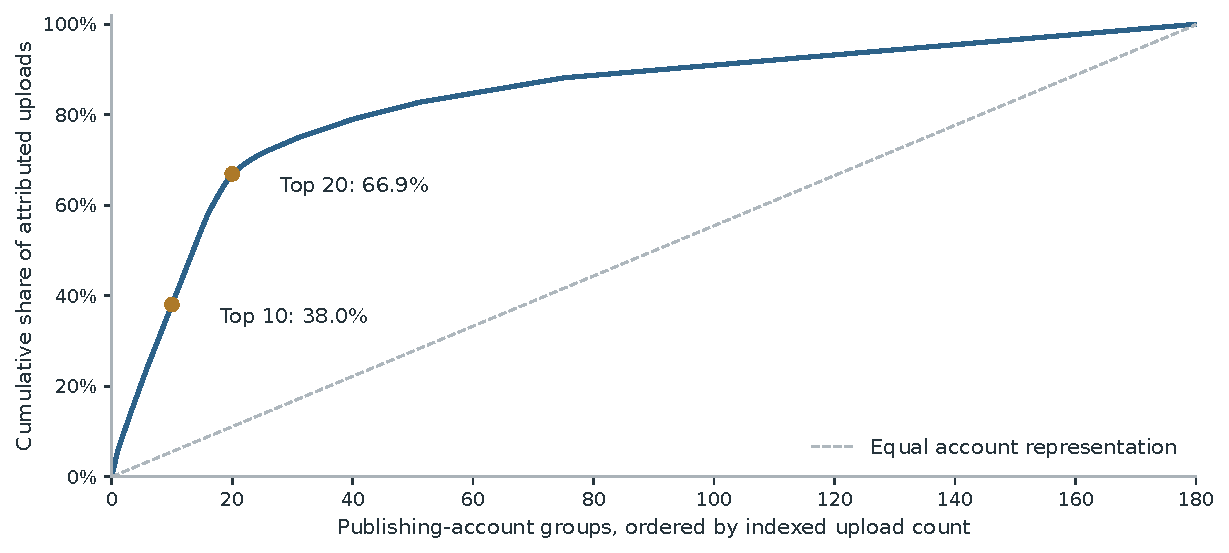
\includegraphics[width=\textwidth]{generated/figures/concentration.pdf}
\caption{Publishing-account concentration among attributed retained uploads. Ranks and cumulative shares describe sample composition. They do not measure followers, views, influence or unique human practitioners.}
\label{fig:concentration}
\end{figure}

\subsection{Caption selection does not favor longer recordings in this snapshot}

The 30 English pilot uploads have median observed length 8.61 minutes, compared with 19.37 minutes in the other 851 indexed uploads with known duration. Restricting the comparison to the pilot's 17 publisher groups gives median 12.04 minutes among 430 other known-duration uploads. The pilot therefore does not have a larger median in either descriptive contrast. This disconfirms the proposed longer-pilot direction, but it is not an estimate of how duration causes caption availability: the pilot selection was purposive and its failures were limited.

\begin{figure}[p]
\centering
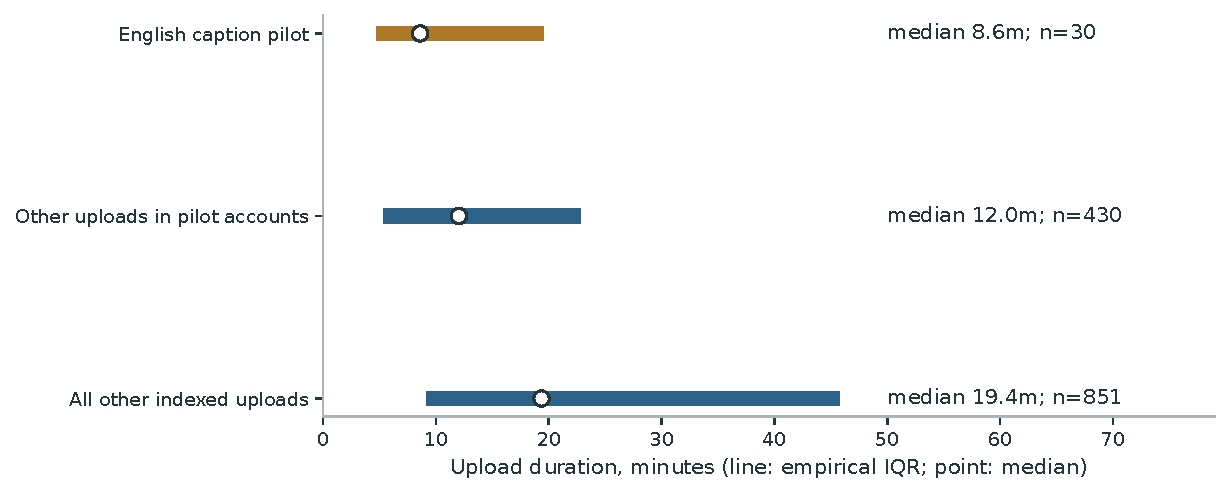
\includegraphics[width=\textwidth]{generated/figures/caption-selection.pdf}
\caption{Observed duration distributions for the English caption pilot, other indexed uploads, and other uploads from pilot publishers. Quartile spans describe observed records; they are not confidence intervals or corrected population estimates.}
\label{fig:caption-selection}
\end{figure}

\subsection{Length and title-keyword framing depend on aggregation}

The title/duration diagnostic uses 702 eligible titles with measured duration: 431 uploads shorter than thirty minutes and 271 of at least thirty minutes. Only 11 accounts meet the paired-account rule on both sides. The pooled direction agrees with the paired-account median direction in two of nine dictionary families. Six paired medians are exactly zero; they must not be described as six reversed effects.

The society/world-events family illustrates an actual sign change: its pooled long-minus-short presence contrast is +4.89 percentage points, whereas the median paired-account contrast is -4.55 points. The compared pools and weighting differ; this is evidence to inspect composition, not a causal duration effect or a full Simpson-paradox identification.

\begin{table}[htbp]
\small\centering
\setlength{\tabcolsep}{4pt}
\begin{tabular}{p{0.39\textwidth}p{0.19\textwidth}p{0.22\textwidth}p{0.08\textwidth}}
\toprule
Dictionary family & Pooled long--short, pp & Median account contrast, pp & Groups \\ \midrule
ET contact \& disclosure & +2.82 & +0.00 & 11 \\
Choice, beliefs \& manifestation & +0.43 & +0.00 & 11 \\
Healing \& wellbeing & -3.26 & +0.00 & 11 \\
Consciousness \& awakening & -0.74 & -4.55 & 11 \\
Energy \& frequency & -5.70 & -3.33 & 11 \\
Collective \& world events & +4.89 & -4.55 & 11 \\
Love \& relationships & -1.21 & +0.00 & 11 \\
Meditation \& practice & -1.12 & +0.00 & 11 \\
Time, dimensions \& realities & +6.50 & +0.00 & 11 \\
\bottomrule
\end{tabular}
\caption{Duration contrast among eligible titles. Families overlap. Per-account estimates use the separately eligible paired-account subset; a zero median is not a directional reversal.}
\end{table}


\begin{figure}[p]
\centering
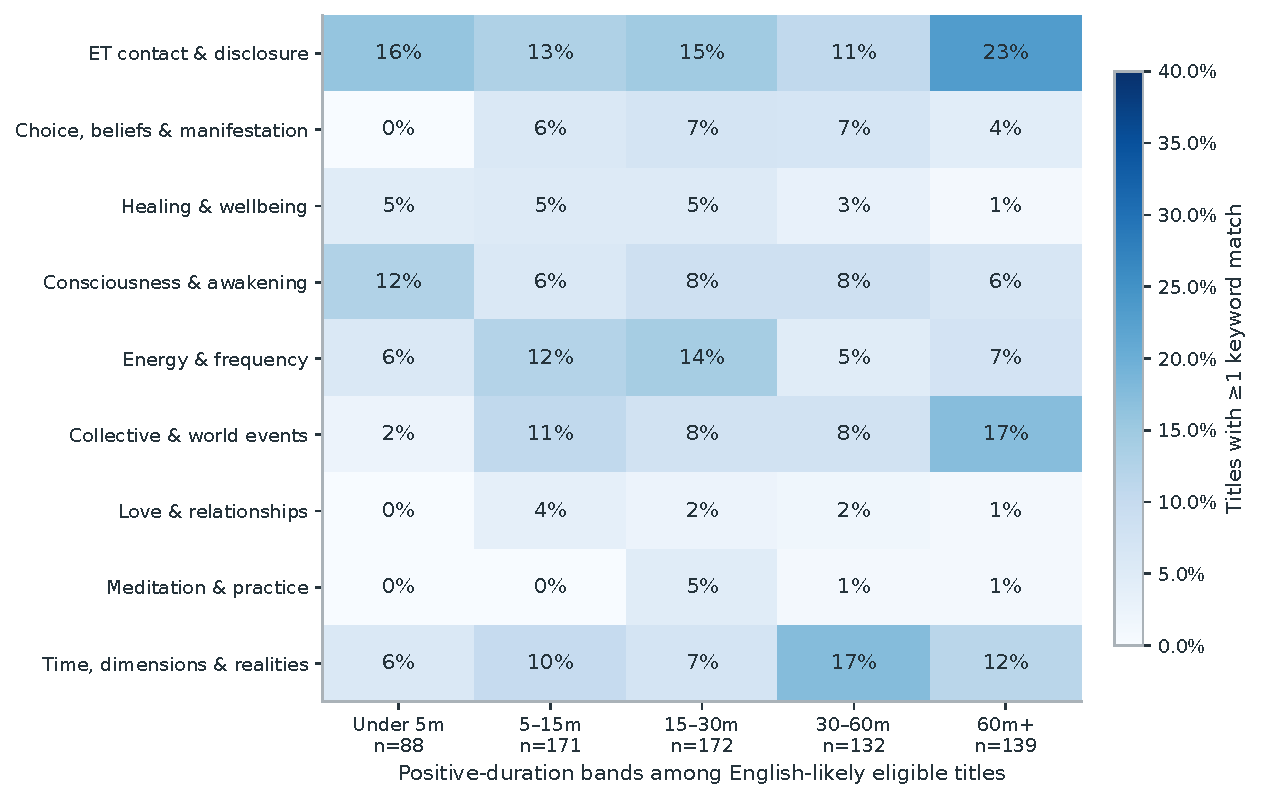
\includegraphics[width=\textwidth]{generated/figures/keyword-duration.pdf}
\caption{Title dictionary presence by observed upload-duration band. Cell denominators are eligible titled uploads with measured duration. Keywords indicate visible framing, not time spent on a theme or validated spoken content.}
\label{fig:keyword-duration}
\end{figure}

\subsection{Publisher resemblance remains a descriptive property of text}

The new upload-pair diagnostic intersects the existing title and caption derivatives, yielding 25 uploads from 14 publishers. This includes groups that do not meet the older two-document account-centroid threshold, so it differs from the prior 22-video/eleven-account centroid comparison. Both new text-layer diagnostics use the same 25 uploads. The mean same-publisher minus different-publisher cosine is 0.154 for captions and 0.229 for titles. The scores describe resemblance under fixed representations, not the probability of shared authorship, an attributed entity or answer agreement.

There are 11 same-publisher and 289 different-publisher upload pairs; 11 accounts have a within-account pair and 3 accounts are singletons. An equal-account sensitivity gives separation 0.153 for captions and 0.229 for titles across 11 eligible focal publishers. Omitting each publisher in turn gives caption separation 0.121--0.179 and title separation 0.186--0.259. These deterministic influence ranges are not confidence intervals.

Caption minus title pooled separation is -0.075; its equal-account analogue is -0.075. Cosine scales are representation-specific, so the difference is a descriptive sensitivity rather than a calibrated amount of semantic or practitioner signal.

The label-shuffle reference permutes publisher labels on the fixed vectors while preserving group sizes (2,000 seed-42 permutations). It is a descriptive negative control, not a population p-value or independent-pair confidence interval. Unresolved original-session reuse, account boilerplate, hosts and publisher formatting remain explanations for a within-publisher advantage. A failure to resemble arbitrary shuffled labels does not isolate a practitioner mechanism.

\begin{figure}[p]
\centering
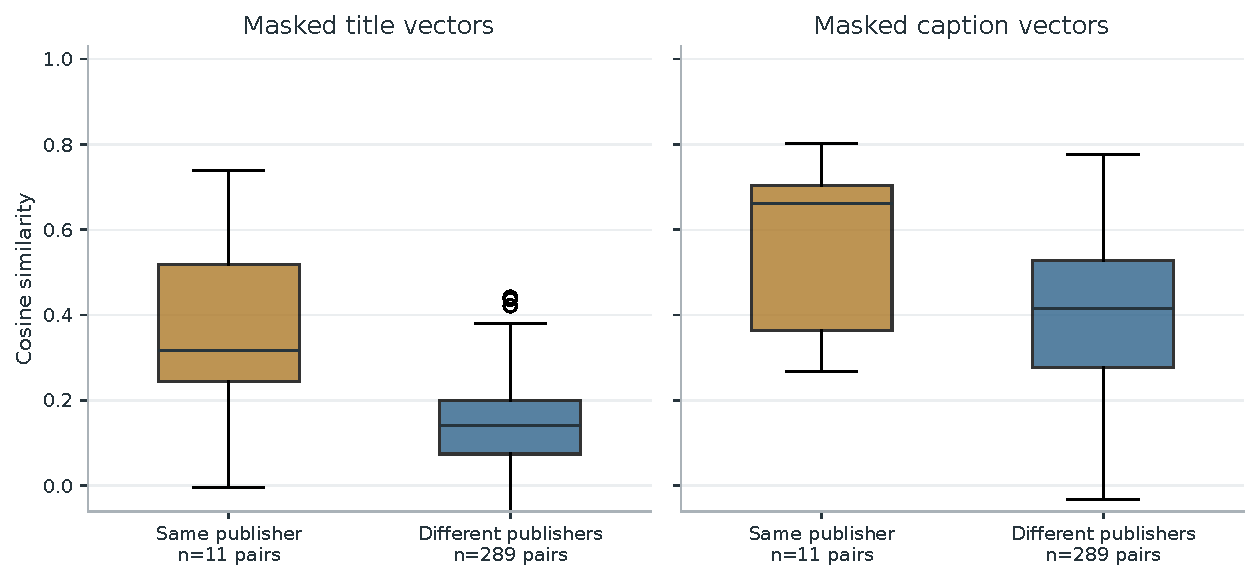
\includegraphics[width=\textwidth]{generated/figures/publisher-similarity.pdf}
\caption{Same- versus different-publisher cosine summaries on fixed title and caption derivatives. Pair entries reuse uploads and are dependent. The new matched upload pool differs from the earlier thresholded centroid cohort.}
\label{fig:publisher-similarity}
\end{figure}

\begin{figure}[p]
\centering
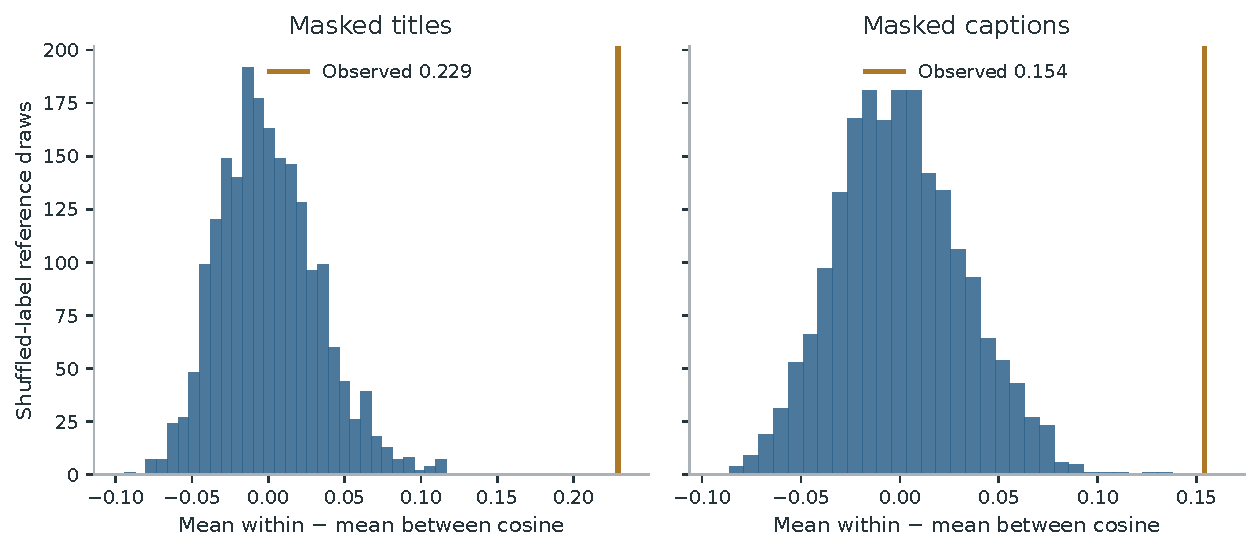
\includegraphics[width=\textwidth]{generated/figures/negative-control.pdf}
\caption{Fixed-vector publisher-label shuffle reference. Labels are permuted with group sizes preserved. The distribution is a descriptive diagnostic, not a population null distribution, a calibrated p-value or evidence about communication origin.}
\label{fig:negative-control}
\end{figure}

\subsection{Repeated title strings are not original-session families}

The new explicitly normalized eligible-title audit finds 2 repeated-string families involving 4 documents among 742 eligible titles; none spans different resolved publishers. Its normalization is different from the inherited embedding-deduplication pipeline. The inherited pipeline's pair-order correlation after its own exclusion rule is 0.992, while raw versus name/genre-masked title rankings correlate at 0.626. These are distinct operations and counts. Neither audit establishes that differently titled uploads are different original performances.

\subsection{Question-answer candidates: useful retrieval, one practitioner context}

The database indexes all 949 retained question/answer-gist entries from 67 Q\&A-bearing digests among 75 source digests. All belong to one Darryl Anka-related practitioner context. They span 27 resolved publisher IDs; 105 candidates lack a resolved publisher ID and remain in 7 inherited-name groups. There are 0 literal transcript turns, 0 verified answer-speaker candidates, and 0 human-reviewed candidates in this layer. The other inherited practitioner candidates do not acquire Q\&A rows merely because they appear in the discovery frame.

\begin{table}[htbp]
\small\centering
\setlength{\tabcolsep}{4pt}
\begin{tabular}{p{0.48\textwidth}p{0.23\textwidth}p{0.15\textwidth}}
\toprule
Source-digest format & Q\&A-bearing uploads & Candidates \\ \midrule
Q\&A only & 5 & 35 \\
clip & 6 & 25 \\
interview with Darryl Anka & 20 & 353 \\
monologue+Q\&A & 36 & 536 \\
\bottomrule
\end{tabular}
\caption{Inherited digest format labels among Q\&A-bearing uploads. Labels are retained source metadata, not a newly validated format taxonomy or answer-speaker annotation.}
\end{table}


\begin{table}[htbp]
\small\centering
\setlength{\tabcolsep}{4pt}
\begin{tabular}{p{0.49\textwidth}p{0.18\textwidth}p{0.2\textwidth}}
\toprule
Q\&A dictionary family & Question matches & Answer-gist matches \\ \midrule
ET contact and disclosure & 155 & 165 \\
Excitement and life direction & 55 & 115 \\
Beliefs, emotions and relationships & 78 & 188 \\
Consciousness and parallel realities & 160 & 348 \\
Channeling and spiritual practices & 89 & 148 \\
Body, health and physical claims & 82 & 265 \\
Time windows and predictions & 31 & 51 \\
History, society and institutions & 42 & 125 \\
\bottomrule
\end{tabular}
\caption{Overlapping keyword matches in question paraphrases and answer gists. Both columns use 949 candidates but different text fields and lengths. Counts are neither validated themes nor measures of agreement.}
\end{table}


There are 936 unique normalized question strings and 11 repeated-string groups. Across distinct uploads, 127 question pairs meet the lexical cosine threshold of 0.40. Excluding identical normalized question wording leaves 112 pairs. These are candidate retrievals, not independent question occurrences or evidence that separate original sessions answered the same prompt.

The retrieval count is sensitive to its exploratory cutoff: increasing question cosine from 0.40 to 0.90 reduces candidate pairs from 127 to 18. At 0.40, the 127 candidate matches occupy 71 distinct upload pairs; the three leading upload pairs supply 30 matches (23.6\%). Concentration can reflect shared questions, reused original material or summary normalization. It is not an observed repost rate or an independent-session count.

\begin{table}[htbp]
\small\centering
\setlength{\tabcolsep}{4pt}
\begin{tabular}{p{0.31\textwidth}p{0.29\textwidth}p{0.27\textwidth}}
\toprule
Minimum question cosine & Candidate question pairs & Distinct upload pairs \\ \midrule
0.40 & 127 & 71 \\
0.50 & 73 & 34 \\
0.60 & 47 & 19 \\
0.70 & 34 & 11 \\
0.80 & 24 & 11 \\
0.90 & 18 & 9 \\
\bottomrule
\end{tabular}
\caption{Exploratory lexical retrieval sensitivity. These thresholds recount the retained question candidates and are not validated equivalence cutoffs. Distinct upload pairs can still share an original performance.}
\end{table}


The summary preview displays 100 of the 127 retained pairs; the complete records are in \texttt{question-pairs.json} and SQLite. Preview truncation is not a lower analyzed denominator. CSV verification/speaker fields retain explicit false values rather than blank strings; null timestamps still mean that no precise turn time is available.

One retrieved pair repeats the digest question \emph{Do we have one life purpose or many?} across two uploads. Its question cosine is 1.000 but its answer-gist cosine is 0.346. The source relation is unresolved: this could involve distinct explanations, summary wording or shared original material. The database correctly marks answer agreement as not assessed rather than converting either score into an agreement verdict.

Twenty deterministically selected digest candidates received model-assisted close reading. The review observes that a contact-oriented question can receive an excitement/formula answer; nested reported speech is not a direct entity turn; precise dates and percentages remain attributed assertions; and a physical-claims keyword is not a clinical validation. The inspected material was the retained question/gist fields. No reviewer listened to the audio or inspected a new transcript in this phase, and the twenty readings do not establish accuracy or inter-rater agreement.

A subsequent purposive paired reading inspects 12 high-question-similarity examples, selecting the first distinct left-question strings in descending cosine order. The model annotations identify compatible paraphrases with low answer-gist cosine, different facets that are not necessarily contradictions, and possible repeated source families. For example, the question of preparing for contact receives passion/formula/vibration advice in both summaries despite low lexical answer similarity. Another pair uses a relative time window versus calendar windows; without original recording dates, it cannot establish chronological drift. Every answer-agreement field remains undetermined. These selected examples refine interpretation of retrieval, not its representative accuracy.
